\section{多FPGA周期精确执行与一致暂停}
\label{sec:midterm-cycle-control}

将DUT划分到多个FPGA后，原本位于片内的部分组合逻辑路径需要通过跨片链路传递信号。由于链路传输需要时间，各分区不能仅根据本地物理时钟独立更新DUT状态，而必须等待当前逻辑周期所需的数据传播完成。此外，各FPGA的执行进度可能不同。当用户请求暂停时，还需要保证所有分区停在同一个DUT逻辑周期，才能获得一致的全局状态。

针对上述问题，REMUS以DUOHUAFEN提出的LI-TDM为基础，实现跨FPGA的周期精确执行，并对每个逻辑周期内的通信流程进行优化，减少不必要的收发操作。同时，在边界数据中加入逻辑周期和传播阶段标识，用于检查通信数据是否按预期顺序到达。在此基础上，REMUS通过接收屏障和共同目标周期协调各分区暂停，为后续分布式状态提取提供一致的逻辑时间边界。

\subsection{基于LI-TDM的跨FPGA周期精确执行及改进}
\label{sec:midterm-li-tdm}

在同步RTL设计中，寄存器在有效时钟边沿更新状态，寄存器之间的组合逻辑则根据当前状态和输入计算下一次更新所需的值。将设计部署到多个FPGA后，部分组合逻辑路径可能跨越FPGA边界。例如，一条路径从FPGA A中的源寄存器出发，经过FPGA B中的组合逻辑，再返回FPGA A中的目标寄存器。在目标寄存器更新之前，信号必须先从A传递到B，经过组合计算后再传回A。

这条组合逻辑路径及其划分后的跨片传输过程如图\ref{fig:midterm-cross-fpga-path-timing}所示。

\begin{figure}[htbp]
    \centering
    % 原图底部包含固定图号，使用trim隐藏，交由LaTeX自动编号。
    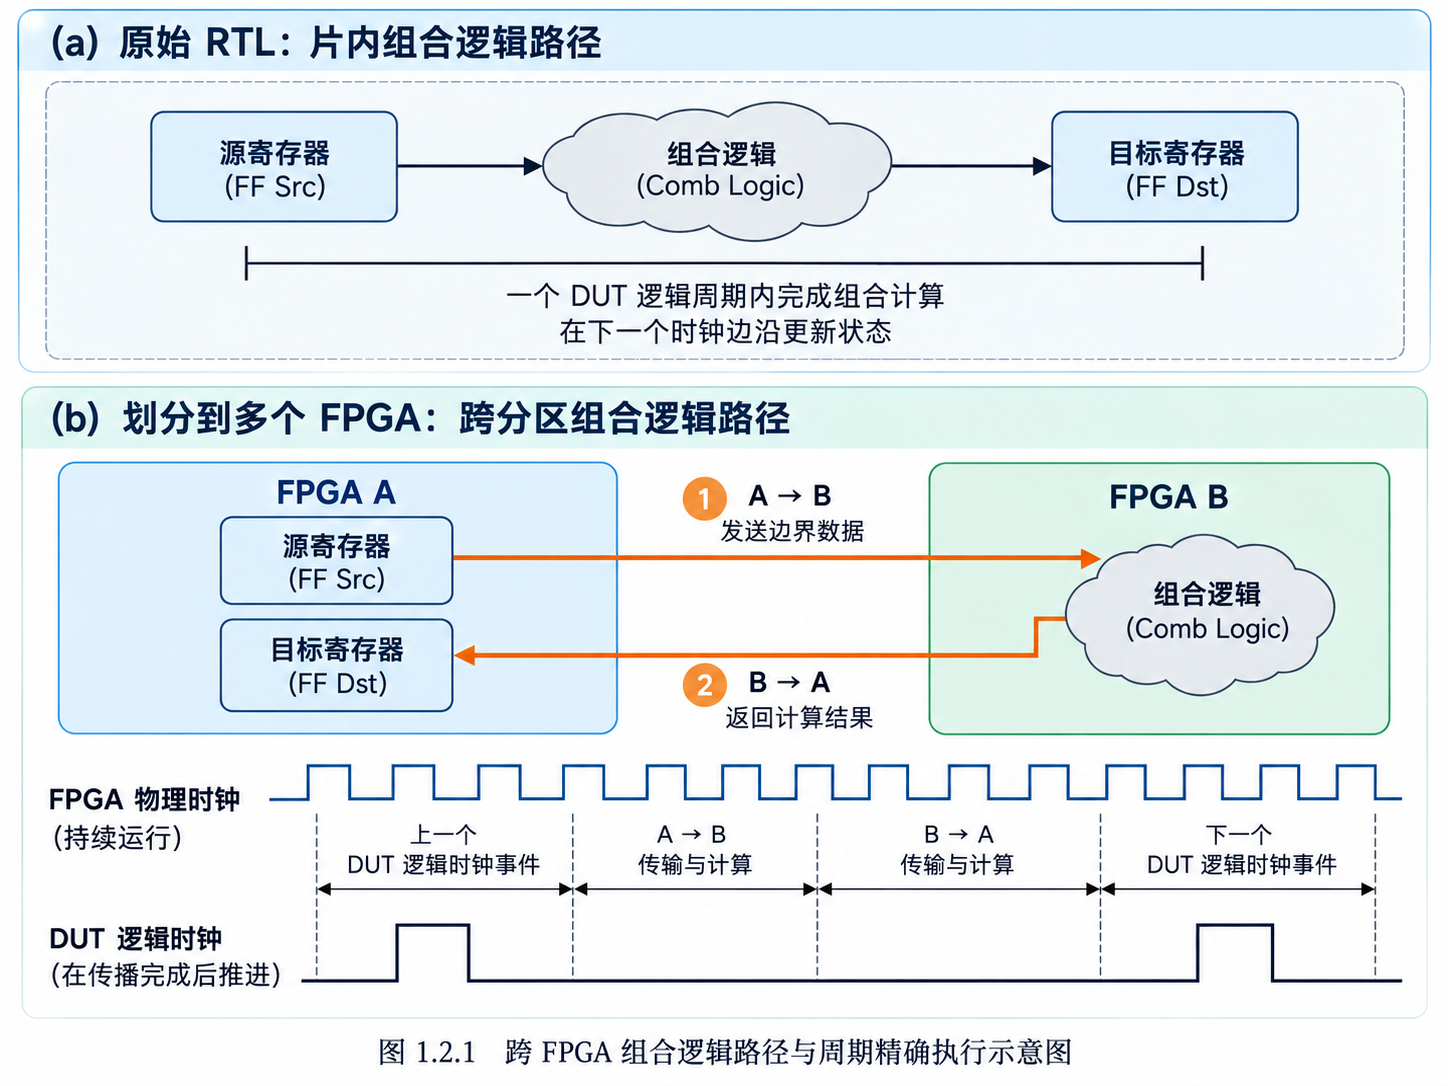
\includegraphics[width=\linewidth,trim=0 3.4cm 0 0,clip]{figure/cross-fpga-combinational-path-timing.png}
    \caption{跨FPGA组合逻辑路径与DUT逻辑时钟推进示意图}
    \label{fig:midterm-cross-fpga-path-timing}
\end{figure}

与片内连接不同，跨FPGA信号需要经过数据打包、物理链路传输和接收重组等过程。如果目标寄存器在数据尚未返回时就更新，得到的结果可能与原始RTL不同。因此，多FPGA周期精确执行的关键，是将跨分区数据传播与DUT逻辑时钟推进协调起来，保证当前周期所需的组合计算完成后再更新时序状态。

DUOHUAFEN提出的LI-TDM机制为跨片执行提供了技术基础\cite{zhu_duohuafen_2024}。该机制结合延迟不敏感（Latency-Insensitive，LI）握手与时分复用（Time-Division Multiplexing，TDM）：前者用于协调跨片数据传输中的等待，后者将较宽的逻辑边界信号分拍映射到有限位宽的物理通信通道。

在LI-TDM中，FPGA物理时钟持续驱动通信与控制逻辑，而DUT逻辑时钟只有在当前周期所需的数据传播完成后才推进。因此，一个DUT逻辑周期可以包含多个FPGA物理时钟周期。跨片通信会延长逻辑周期的实际执行时间，但不应改变DUT在该周期的状态更新结果。

\paragraph{跨分区传播过程与路径切割数}

LI-TDM通过多个传播阶段完成一个DUT逻辑周期内的组合计算。原有机制在每个阶段依次等待接收边界数据、计算本地组合逻辑，再将结果发送给其他分区。数据通过这些阶段沿跨分区组合路径逐步传播。

对于前述FPGA A到B再返回A的例子，A首先向B发送源寄存器产生的边界数据；B收到数据后完成相应的组合计算，再将结果发回A；A获得返回的数据后，才能确定目标寄存器的下一状态。虽然系统只有两个FPGA，但这条组合路径包含两次跨分区传播。

不同电路划分所需的传播阶段数并不相同。已有电路划分研究使用路径切割数（path-cut number）表示一条信号路径中被划分切断的连接数\cite{sait_evolutionary_2002}。设合法组合路径中的最大路径切割数为$N_{\mathrm{cut}}$，在本文采用的LI-TDM执行方式下，一个DUT逻辑周期所需的传播阶段数为$S=N_{\mathrm{cut}}+1$。例如，前述A→B→A的组合路径有两次跨分区连接，需要三个分区内计算阶段。路径切割数反映逻辑依赖跨越分区边界的次数，并不等于物理网络中的路由跳数。具体定义与计算方法见第\ref{sec:midterm-path-cut}节。

\paragraph{首尾传播阶段的收发优化}

REMUS沿用LI-TDM分阶段传播的基本机制，但对每个逻辑周期的首尾阶段进行了优化。

原有流程在首阶段也会先等待接收数据。然而，在DUT逻辑时钟刚刚更新后，各分区已经获得当前周期的本地寄存器值，可以直接计算并发送由这些状态决定的初始边界数据，不必先等待新一轮跨片接收。对于仍依赖其他分区输入的组合逻辑，其结果会随着后续阶段的数据到达而逐步确定。因此，首阶段省去的是跨片接收等待，而非所有本地输入与模型交互条件。

中间传播阶段保持原有流程：接收边界数据、完成本地组合计算，再将结果发送给后续依赖的分区。

在最后一个传播阶段，所需的边界数据已经到达，分区完成相应组合计算后，当前周期的跨分区依赖得到满足，可以推进DUT逻辑时钟。由于不再需要执行下一传播阶段，此时也无须再次发送计算结果。

因此，REMUS将首阶段调整为“计算、发送”，中间阶段保持“接收、计算、发送”，末阶段则调整为“接收、计算、更新DUT逻辑时钟”。两种流程的区别如图\ref{fig:midterm-li-tdm-stage-optimization}和表\ref{tab:midterm-li-tdm-stages}所示。

\begin{figure}[htbp]
    \centering
    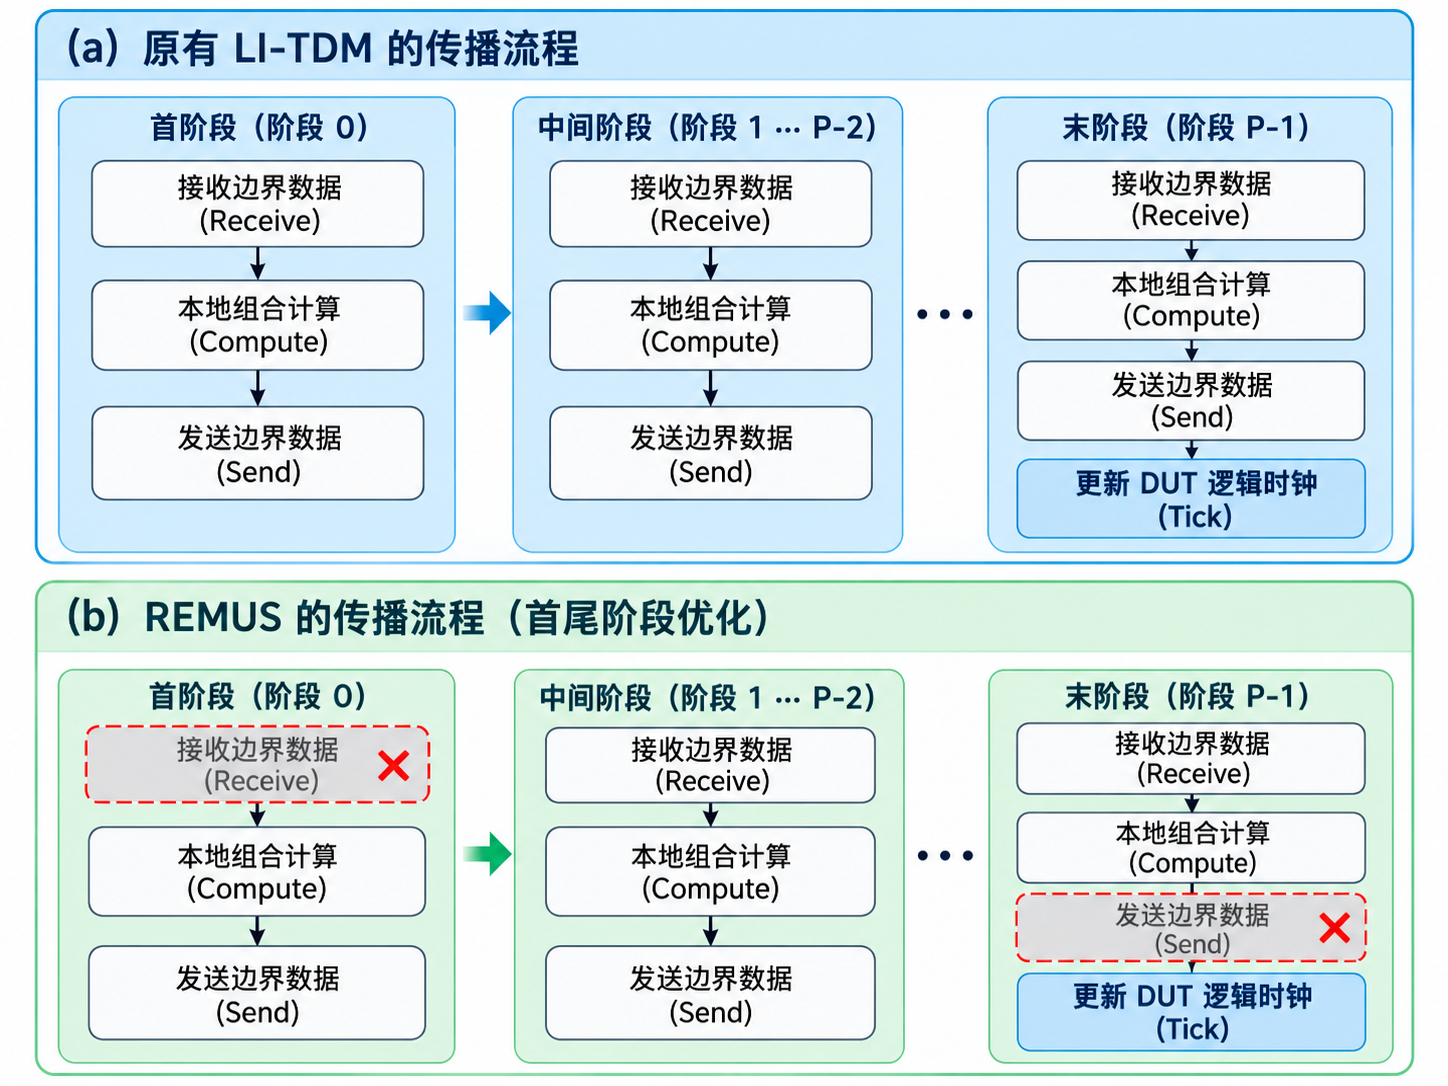
\includegraphics[width=\linewidth]{figure/li-tdm-propagation-stage-optimization.png}
    \caption{LI-TDM原始传播流程与REMUS首尾阶段收发优化对比}
    \label{fig:midterm-li-tdm-stage-optimization}
\end{figure}

\begin{table}[htbp]
    \centering
    \caption{LI-TDM传播流程与REMUS首尾阶段改进}
    \label{tab:midterm-li-tdm-stages}
    \small
    \renewcommand{\arraystretch}{1.25}
    \begin{tabularx}{\linewidth}{@{}l>{\raggedright\arraybackslash}X>{\raggedright\arraybackslash}X@{}}
        \toprule
        传播阶段 & 原有LI-TDM & REMUS改进后 \\
        \midrule
        首阶段 & 接收、计算、发送 & 计算、发送 \\
        中间阶段 & 接收、计算、发送 & 接收、计算、发送 \\
        末阶段 & 接收、计算、发送、更新时钟 & 接收、计算、更新时钟 \\
        \bottomrule
    \end{tabularx}
\end{table}

与原有流程相比，REMUS在每个DUT逻辑周期内省去首阶段的一次接收和末阶段的一次发送，从而减少冗余通信与等待。该优化利用的是逻辑周期首尾不同的数据依赖条件，没有改变电路划分结果，也没有省略必须完成的组合逻辑传播。

这一改进能够降低每个逻辑周期的通信开销，但实际运行性能仍受到最大路径切割数所决定的传播阶段数、边界数据量、链路延迟及本地模型响应时间等因素影响。具体性能改善需要通过后续实验评估。

\paragraph{基于周期与传播阶段标识的通信序列一致性检查}

除了减少通信开销，跨FPGA执行还需要保证各分区接收到正确的边界数据。一个DUT逻辑周期可能包含多轮跨片传输。如果通信控制、缓存或调度逻辑出现缺陷，数据可能发生丢失、重复或乱序。错误数据一旦参与组合计算，可能经过多个逻辑周期才表现为程序输出异常，难以定位最初出错的位置。

为此，REMUS在边界数据中加入逻辑周期与传播阶段标识。逻辑周期标识用于区分数据所属的DUT周期，传播阶段标识则用于区分同一周期内不同的数据传播过程。

接收数据时，分区根据当前执行进度及协议规定的收发阶段对应关系，判断数据是否属于预期的执行上下文。这里并不要求发送端与接收端的阶段编号简单相等，而是检查两者是否满足协议定义的对应关系。只有检查通过的数据才能参与后续组合计算。

当数据标识与预期不符时，一致性检查可以报告对应的逻辑周期和传播阶段，使错误更早暴露在通信接口处，而不必等到DUT程序执行失败后再定位。这有助于排查跨分区通信及控制逻辑中的时序问题。

需要指出的是，该机制用于检测和定位通信序列异常，不提供自动重传或乱序重排功能。对于标识相同的重复数据，或者数据缺失后没有新的数据到达等情况，还需要结合收发计数、超时等检查方式。

通过上述改进，REMUS在保留LI-TDM周期精确执行机制的基础上，减少了首尾阶段的冗余收发，并增强了通信过程的可诊断性。

周期精确执行并不要求所有FPGA在任意物理时刻都处于同一个DUT逻辑周期。各分区可以因通信等待而具有不同的执行进度，只要各逻辑周期的计算与状态更新保持正确即可。然而，当系统需要提取全局状态时，就必须使所有分区停在相同的逻辑周期。这也是下一节研究多FPGA一致暂停机制的原因。

\subsection{多FPGA一致暂停机制}
\label{sec:midterm-global-pause}

周期精确执行保证了跨分区计算的正确性，但不意味着各FPGA在任意物理时刻都处于同一个DUT逻辑周期。由于控制请求的传输和分区间的通信等待不同，主机发出暂停指令后，各分区可能停在不同周期。此时，即使每个分区都已停止，其局部状态也无法直接组成同一逻辑时刻的全局状态。

例如，两个分区收到暂停请求时，FPGA A可能已完成第42个逻辑周期，FPGA B则只完成了第41个周期。如果立即分别停止，得到的状态便相差一个逻辑周期。REMUS不要求暂停请求同时到达，而是先确定各分区的执行进度，再使其继续运行到同一个目标周期。整个过程中，DUT逻辑时钟可以停止推进，但通信及主机控制逻辑仍由FPGA物理时钟驱动。

REMUS复用扫描链控制器中的逻辑周期计数、运行状态和定步执行能力，并增加同步屏障的请求与确认接口。逻辑周期计数记录已完成的DUT周期数；剩余步数寄存器规定还需执行的周期数。两者配合，使主机能够将不同进度的分区协调到相同的逻辑周期边界。具体过程分为稳定采样、目标配置、定步执行和最终检查四步。

\paragraph{接收屏障与稳定进度采样}

主机首先向全部分区发出同步屏障请求。分区收到请求后，完成进入下一接收边界前所需的动作，并停留在该接收边界，向主机返回屏障确认。屏障确认不要求本阶段待接收数据已到达，因此分区可以暂时保持在接收位置，而不必等待其他分区继续推进。

只有收齐所有屏障确认后，主机才逐个读取逻辑周期计数。此时，各分区的传播进度已固定，计数不会在读取期间继续变化，因而能够作为后续协调的起点。

需要区分的是，接收屏障只是为主机提供稳定的采样与配置位置，并不代表DUT已经在有效的全局状态上暂停。分区之间仍可能存在周期差异，通信缓存中也可能保留尚未使用的数据。后续必须完成必要的传播和状态更新，才能形成真正的一致暂停点。

\paragraph{共同目标周期与定步执行}

设系统共有$N$个分区，分区$i$在接收屏障处已完成的逻辑周期数为$c_i$。为了使所有分区都能够向前执行，并完成屏障处尚未结束的周期，主机将共同暂停目标设为最领先分区当前周期之后的一个周期：
\begin{equation}
    T = \max_{0 \leq i < N} c_i + 1.
    \label{eq:midterm-pause-target}
\end{equation}
随后，主机为各分区配置剩余执行步数：
\begin{equation}
    s_i = T - c_i, \qquad 0 \leq i < N.
    \label{eq:midterm-pause-steps}
\end{equation}
这里的一步表示完成一个DUT逻辑周期，而非一个FPGA物理时钟周期。由于$T$大于所有已采样的$c_i$，各分区都至少需要再执行一步，不必回退已经更新的DUT状态。

仍以前述双FPGA为例。若在接收屏障处采样到$c_A=42$、$c_B=41$，则$T=43$。主机分别配置$s_A=1$、$s_B=2$：FPGA A再完成一个逻辑周期，FPGA B再完成两个逻辑周期，最终均停在第43个周期结束的位置。这说明一致暂停不要求两个FPGA执行相同的剩余步数，而要求它们到达相同的终点。

双FPGA一致暂停的协调时序如图\ref{fig:midterm-dual-fpga-pause-timing}所示。

\begin{figure}[htbp]
    \centering
    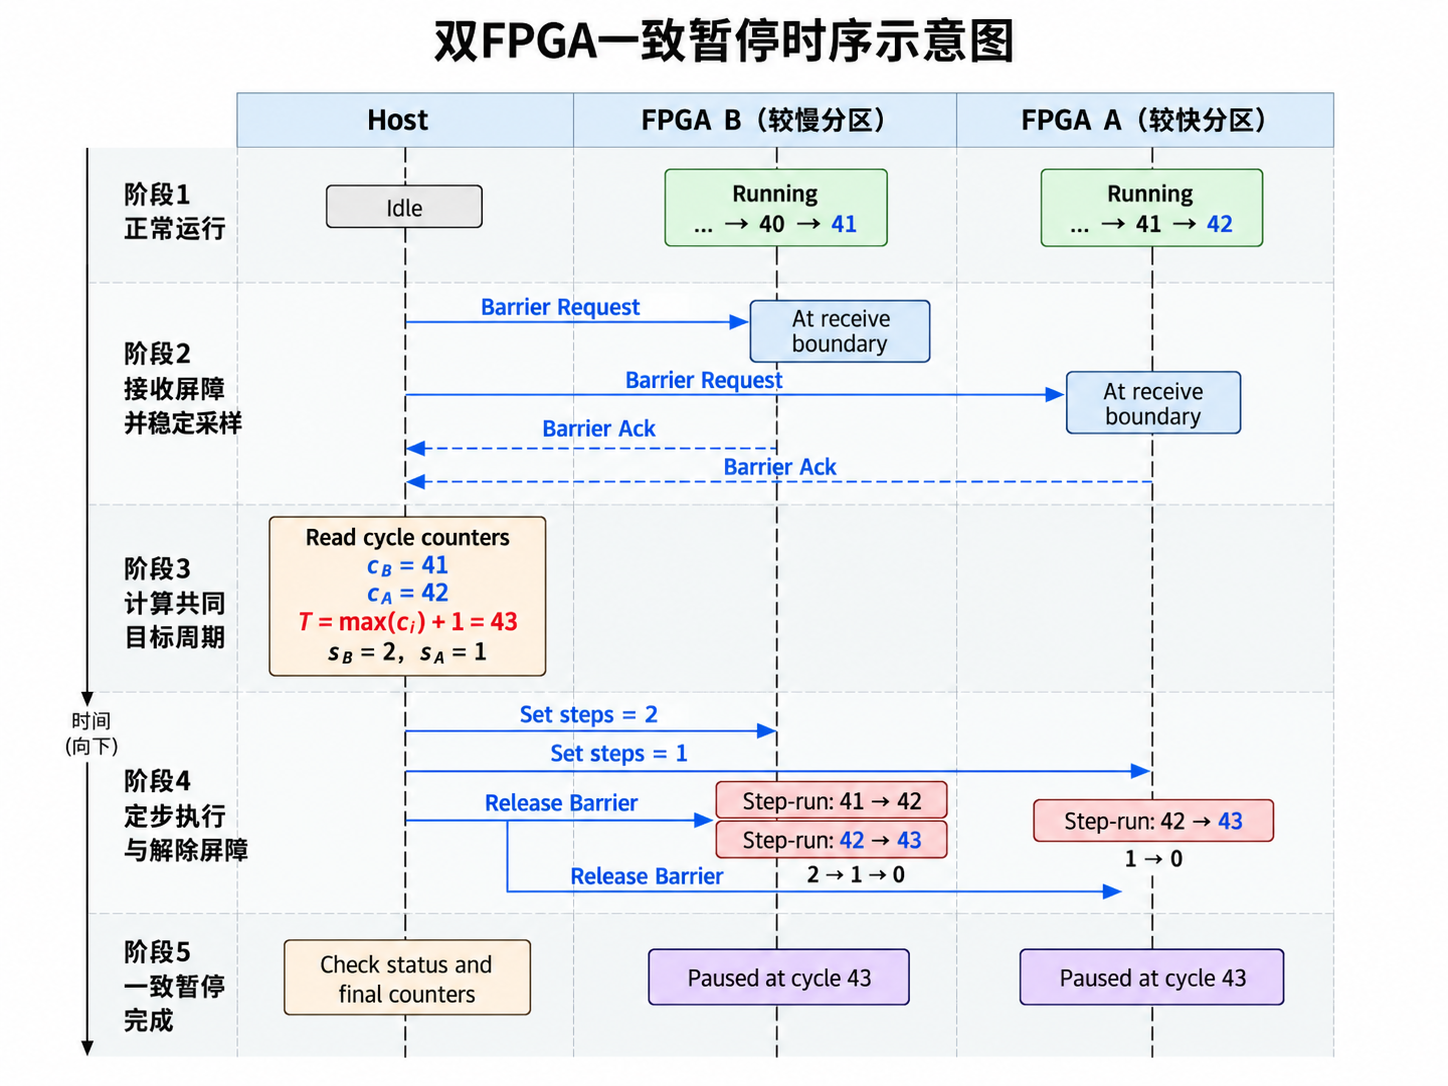
\includegraphics[width=\linewidth]{figure/dual-fpga-consistent-pause-timing.png}
    \caption{双FPGA一致暂停的屏障协调与共同目标周期示意图}
    \label{fig:midterm-dual-fpga-pause-timing}
\end{figure}

所有步数均在屏障保持期间写入。配置完成后，主机按已采样进度从落后到领先的顺序解除屏障，上例中先解除FPGA B，再解除FPGA A。解除屏障只允许分区继续参与原有的LI-TDM握手，并不绕过跨分区数据依赖；各分区在完成所需的组合传播后推进DUT逻辑周期，每完成一个周期便递减剩余步数。采用这一释放顺序，是为了使落后分区先获得继续传播的机会；在不同拓扑中的等待关系和正确性仍需结合实际通信协议验证。

\paragraph{暂停完成判定}

当剩余步数减至零时，各分区停止DUT正常执行。主机随后检查全部分区的运行状态、暂停处理状态和最终逻辑周期计数。只有各分区均已停止，且计数都等于目标$T$，才向上层报告全局一致暂停完成。

为避免将通信等待或协调失败误判为成功，进入接收屏障和等待最终暂停均设置等待上限。对周期目标溢出、步数超出寄存器范围以及最终计数不一致等情况，主机显式报告错误。

\paragraph{全局暂停点的状态要求}

周期计数相等说明各分区到达了相同的逻辑时间边界，但它本身不能证明内部状态正确。有效的一致暂停还要求到达目标周期所需的组合计算和跨分区传播已完成，且DUT时序状态不会在暂停后继续因正常执行而更新。接收屏障确认或单个发送接口完成握手，都不能代替这些条件。

因此，REMUS的验证需要同时检查两件事：首先，所有分区是否停在相同的目标周期；其次，暂停后的分布式状态是否与未划分DUT在该周期的参考状态一致。前者确认暂停位置，后者检查暂停点的功能正确性。一致暂停解决的是全局状态的时间边界问题；状态覆盖、映射、恢复和重放仍由后续分布式状态管理机制处理。

\subsection{周期精确执行与一致暂停的验证方法及结果}
\label{sec:midterm-cycle-cosim}

本节通过Cosim对照检查划分前后的DUT行为，以及不同执行进度的分区能否在同一逻辑周期正确暂停。现阶段已验证划分后的DUT程序执行结果正确，一致暂停后比对寄存器数值与预期相同，周期级事件的连续对照仍需完善。

\subsubsection{验证目标与实验设置}

以PicoRV32和香山昆明湖（KMH）为验证对象，比较为划分的设计与采用LI-TDM的多分区执行。下面以PicoRV32为例，实验采用未分区的单Part Cosim作为参考，与双Part Cosim运行相同的手写裸机程序，并采用相同的64周期复位流程。单Part提供同周期参考状态，双Part用于检查跨分区执行和全局暂停。该对照不同于物理单板、双板上板实验，后者的检查点结果在第\ref{sec:midterm-board-checkpoint-comparison}节单独说明。

对照以DUT逻辑周期为基准。由于跨片通信可以占用多个FPGA物理时钟周期，不能直接用两种仿真消耗的物理时钟数判断执行语义是否一致。周期精确性通过输出与周期级事件对照验证，暂停正确性则通过周期计数和暂停点状态共同检查。

% PicoRV32案例来源：experiments/picorv32-cosim-cycle-state.md及对应原图。
% TODO(复现配置)：补DUT/工具版本、初始内存及完整输入配置、划分产物标识；
% KMH已有定性对照另补具体程序、周期和状态范围，不用PicoRV32案例代替。

\subsubsection{周期精确执行的正确性验证}

首先，在单体参考环境和多分区Cosim中运行相同的软件程序，并在对应的执行进度下比较程序输出。已有PicoRV32与KMH测试在所比较的执行区间内得到相同的程序输出。这一对照检查了跨分区执行的可观察结果，但程序输出相同并不足以证明每个逻辑周期的内部行为都一致。因此还通过检查点机制，比对相同时刻点的寄存器数值。

PicoRV32具体案例中，两种配置均在复位64周期后释放复位，先运行至2048周期并保存检查点。此后，单Part指定运行到42080周期，双Part继续执行并通过全局暂停停在42080周期。两侧终端均输出\texttt{Sieve benchmark}，随后显示\texttt{Primes:}及2至61的18个素数，截图可见的输出前缀一致。这里的运行目标是绝对逻辑周期，因此64至2048推进1984周期，2048至42080推进40032周期。该记录检查了相同逻辑执行位置的可观察结果。

为了更直接地检验周期精确性，后续通过检查点机制，保存了单体参考的与多分区Cosim在相同逻辑周期下的检查点，通过比对相同寄存器变量的数值，可以证明该周期多分区Cosim的执行与单体参考是一致的，详见下一节。


\subsubsection{一致暂停的正确性验证}

在多分区Cosim运行过程中发出暂停请求，记录各分区进入接收屏障时的已完成逻辑周期数$c_i$。按照式\eqref{eq:midterm-pause-target}计算共同目标周期$T$，再由式\eqref{eq:midterm-pause-steps}确定各分区的剩余执行步数$s_i$。解除屏障并等待暂停结束后，检查所有分区是否停止，以及最终周期计数是否均等于$T$。

除正常执行下的暂停请求外，还应在不同物理触发时刻和传播阶段发出请求，并通过可控的通信等待构造不同的分区进度差。这些场景用于检查屏障采样、差异化步进和最终停止条件是否正确，不通过修改周期计数或DUT内部状态人为制造结果。

周期计数相同只能证明暂停位置一致。为检查暂停状态的正确性，还需将单体RTL推进到相同的逻辑周期，按原始DUT与各分区的状态映射关系比较相应寄存器和存储状态，并记录比较范围。状态提取与Global Snapshot的构建方法在1.3节进一步讨论。

已有PicoRV32和KMH的Cosim实验中，各分区在暂停后到达相同周期，实际比较的内部状态与同周期单体参考相同。板级日志进一步记录了双Part的同步暂停：PicoRV32的23条摘录耗时为0.803--0.925 ms，KMH的一条记录为1.047 ms。该时间从主机发起屏障请求前计至各Part停止且最终tick检查完成，体现Host可见的协调开销；它不是FPGA内部纯屏障延迟，也不能代替暂停状态对照。详细板级案例见第\ref{sec:midterm-prototype-observation}节。

在上述PicoRV32案例中，单Part通过目标周期自动停止，双Part通过全局暂停停止，随后均保存42080周期检查点，并检查相同寄存器和SRAM变量的数值是否相等。图\ref{fig:midterm-single-part-state-comparison}展示两侧解码结果，表\ref{tab:midterm-single-part-state-comparison}列出共同可见的四个对应寄存器，其位宽与数值均一致。因此，本例不仅检查最终周期计数，还用单Part参考检查了双Part暂停后的选定内部状态。

\begin{figure}[htbp]
    \centering
    % 原图96 dpi，左右分界约在x=1028像素；仅以TeX裁切分两行显示，保留原图。
    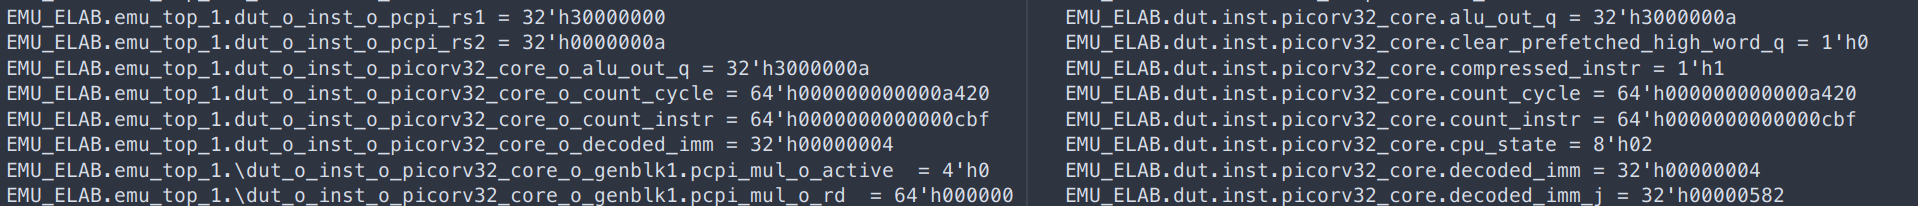
\includegraphics[width=\linewidth,trim=0 0 668bp 0,clip]{experiments/figure/single-vs-part2.png}
    \par\smallskip
    {\small （a）双Part检查点中的处理器状态}
    \par\medskip
    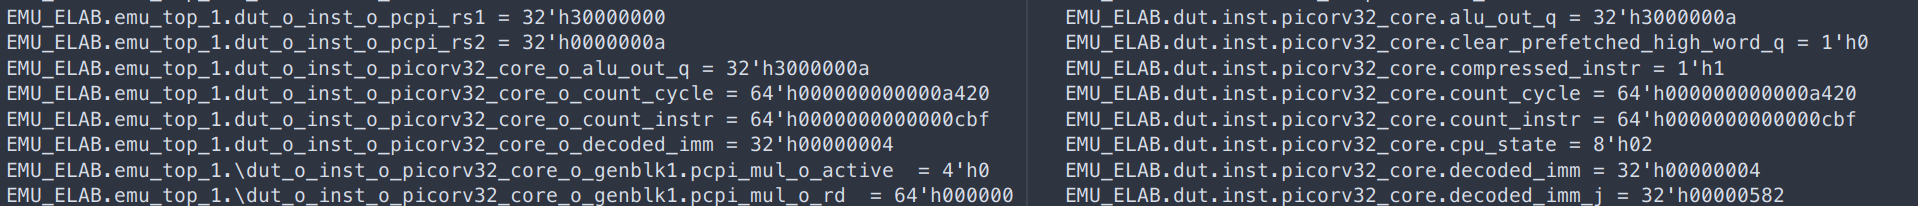
\includegraphics[width=\linewidth,trim=771bp 0 0 0,clip]{experiments/figure/single-vs-part2.png}
    \par\smallskip
    {\small （b）单Part检查点中的处理器状态}
    \caption{PicoRV32在42080周期的单Part与双Part Cosim检查点对照}
    \label{fig:midterm-single-part-state-comparison}
\end{figure}

\begin{table}[htbp]
    \centering
    \caption{42080周期检查点中选定对应寄存器的比较}
    \label{tab:midterm-single-part-state-comparison}
    \small
    \begin{tabular}{@{}lcll@{}}
        \toprule
        寄存器                   & 位宽/bit & 单Part值                    & 双Part值                    \\
        \midrule
        \texttt{alu\_out\_q}  & 32     & \texttt{3000000a}         & \texttt{3000000a}         \\
        \texttt{count\_cycle} & 64     & \texttt{000000000000a420} & \texttt{000000000000a420} \\
        \texttt{count\_instr} & 64     & \texttt{0000000000000cbf} & \texttt{0000000000000cbf} \\
        \texttt{decoded\_imm} & 32     & \texttt{00000004}         & \texttt{00000004}         \\
        \bottomrule
    \end{tabular}
    \par\smallskip
    {\footnotesize 数值均为十六进制，位宽单列。}
\end{table}

对应寄存器的层次名称不同，是因为自适应划分选择性展开原始层次，再将单元重新打包到各Part。以\texttt{alu\_out\_q}为例，对应路径如下，两者均省略共同的\texttt{EMU\_ELAB}根层次：
\begin{quote}
    \small
    单Part：\texttt{dut.inst.picorv32\_core.alu\_out\_q}\\
    双Part：\texttt{emu\_top\_1.dut\_0\_inst\_0\_picorv32\_core\_0\_alu\_out\_q}
\end{quote}
比较时按原始逻辑对象和状态映射建立对应，而非要求名称字符串相同。表中的\texttt{count\_cycle}是DUT内部计数器，其值\texttt{0xa420}为42016，等于$42080-64$，与复位期间该计数器被清零的行为相符。

% 已补42080周期四项寄存器对照；count_cycle语义见PicoRV32源码的resetn更新。
% TODO(暂停协调日志)：仍补各Part的c_i/T/s_i及最终tick；现有运行图
% 只显示Driver最终tick，不能据此编造屏障采样值或差异化步数。
% TODO(暂停鲁棒性)：补充不同触发时刻、传播阶段和受控链路等待场景，
% 包括成功率、超时与异常场景；未执行的场景不得写成已通过。
